\documentclass[12pt, a4paper, twoside, article]{memoir}
\usepackage[a4paper, total={6.5in, 8in}]{geometry}
\usepackage[utf8]{inputenc}
\usepackage[english]{babel}
\usepackage[T1]{fontenc}
\usepackage[final]{microtype}
\usepackage{amsmath,amssymb}
\usepackage{bm}
\usepackage{amsthm}
\usepackage{mathtools}
\usepackage{listings}
\usepackage{graphicx}
\usepackage{amsmath}
\makeatletter
\renewcommand*\env@matrix[1][*\c@MaxMatrixCols c]{%
	\hskip -\arraycolsep
	\let\@ifnextchar\new@ifnextchar
	\array{#1}}
\makeatother
\usepackage[colorlinks=true,linkcolor=blue,urlcolor=black]{hyperref}
\usepackage{bookmark}
\DeclareMathSymbol{*}{\mathbin}{symbols}{"01}
\usepackage{color}

\usepackage[sc]{mathpazo}
\renewcommand{\ttdefault}{txtt}
\linespread{1.06}
\renewcommand{\chapnamefont}{\large\em}
\newcommand{\regi}[1]{ %
	{%
		\centering
		\em #1
		\par
	}
}

\setcounter{tocdepth}{3}
\setcounter{secnumdepth}{3}

% Fancy chapters
\usepackage{tikz}
\makechapterstyle{box}{
	\renewcommand*{\printchaptername}{}
	\renewcommand*{\chapnumfont}{\HUGE\bfseries}
	\renewcommand*{\printchapternum}{
		\flushright
		\begin{tikzpicture}
			\draw[fill,color=black] (0,0) rectangle (2cm,2cm);
			\draw[color=white] (1cm,1cm) node { \chapnumfont\thechapter };
		\end{tikzpicture}
	}
	\renewcommand*{\chaptitlefont}{\HUGE\bfseries}
	\renewcommand*{\printchaptertitle}[1]{\flushright\chaptitlefont##1}
}
\chapterstyle{box}



% Fancy headers
\usepackage{fancyhdr}

\pagestyle{fancy}
\fancyhf{}
\fancyhead[LE,RO]{}
\fancyhead[RE,LO]{\textsc{Marc Breiner Sørensen}}
\fancyfoot[RE,CO]{\thepage}
\fancyfoot[LE,RO]{ \tiny\leftmark}

\renewcommand{\headrulewidth}{2pt}
\renewcommand{\footrulewidth}{1pt}


% Fancy breadtext
%\usepackage{ebgaramond, fontspec}
%\setmainfont{EB Garamond}
%\renewcommand{\familydefault}{\ebgaramond}
\usepackage {xcolor}

\title{\color{white}\textsc{\textbf{STEP} \\ \normalsize Subtitle}}	
\author{\color{white}\normalsize Student: \textbf{\textsc{Marc Breiner Sørensen
			\#\small\textsf{201708238}}}\\
	\color{white}\normalsize Supervisors: \textbf{Hans Kjeldsen} \& \textbf{Mads Fredslund Andersen}\\
	\color{white}\normalsize Institut for Fysik og Astronomi, Aarhus Universitet}
\date{\color{white}\textsc{\textsf{\today}}}

\usepackage{tcolorbox}

\usepackage{eso-pic,graphicx}
% Multi-file preamble stuff
\graphicspath{{images/}}
\usepackage{subfiles} % Best loaded last in the preamble
\begin{document}
	\AddToShipoutPictureBG*{\centering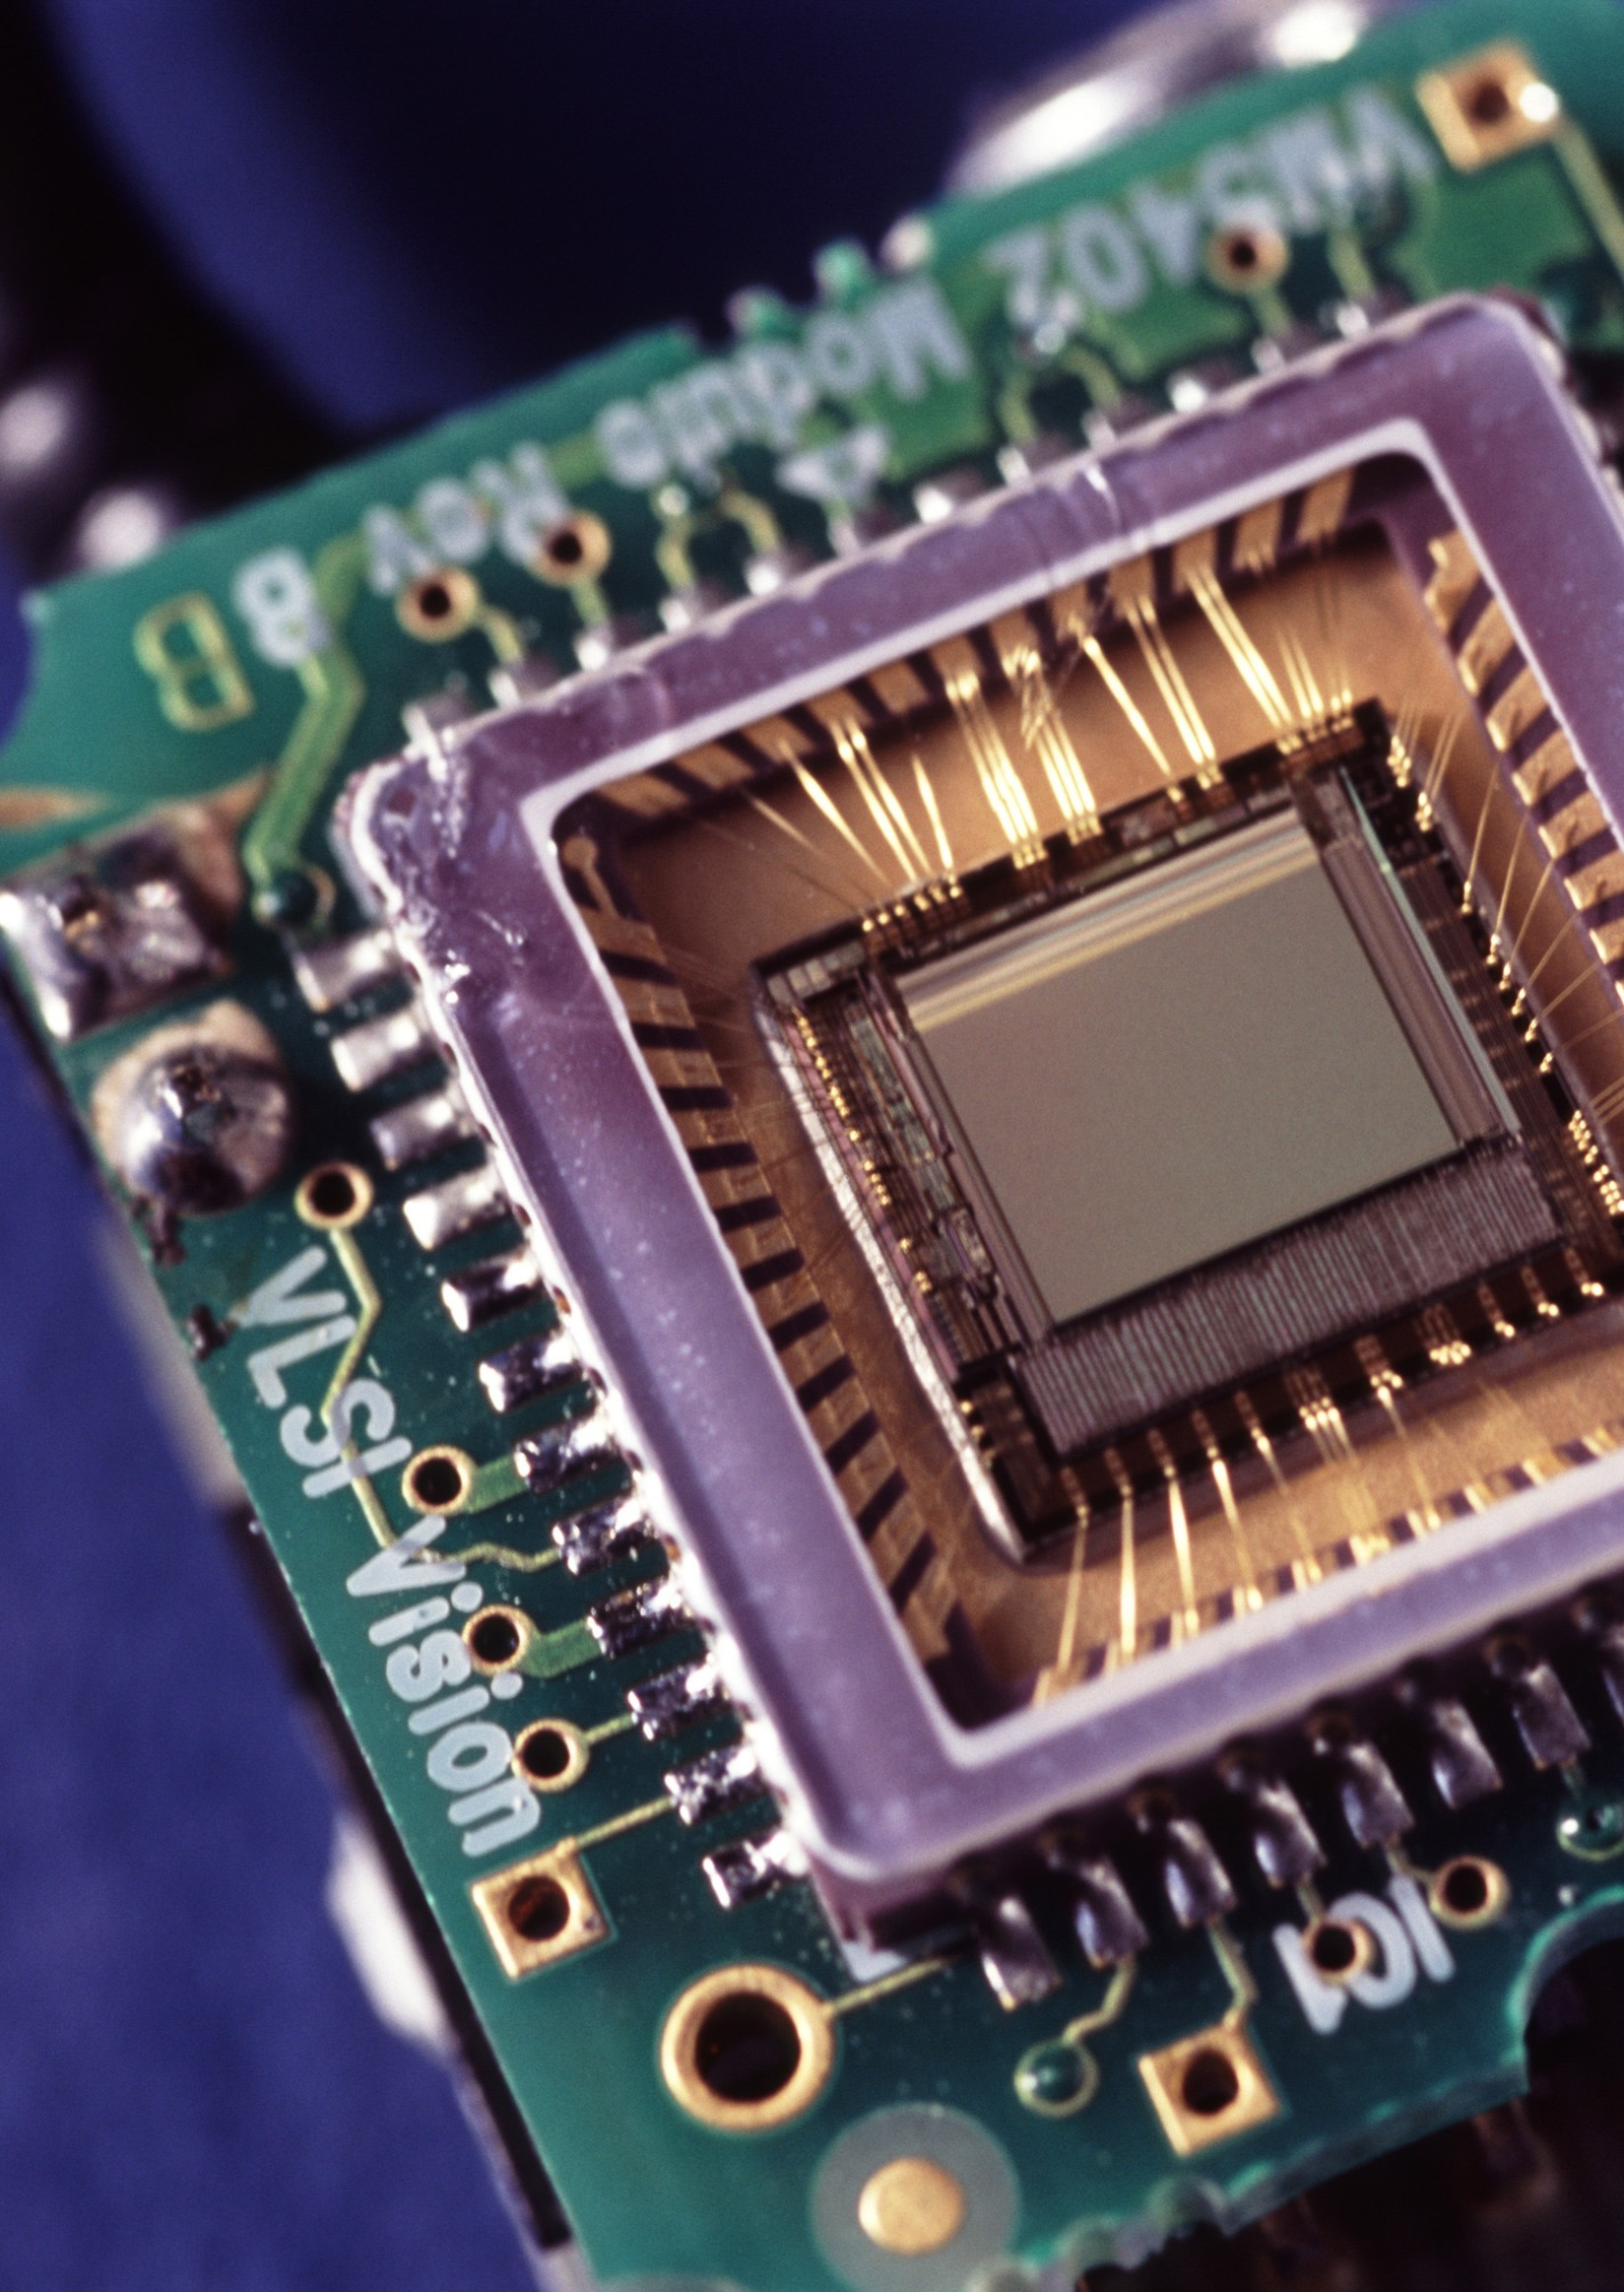
\includegraphics[width=\paperwidth,height=\paperheight]{ccd_sensor_bg.jpg}};
	\begin{tcolorbox}[colback = black, colframe = black, sharpish corners]
	\maketitle
\end{tcolorbox}

	%\begin{figure}[h!]
	%	\centering
		%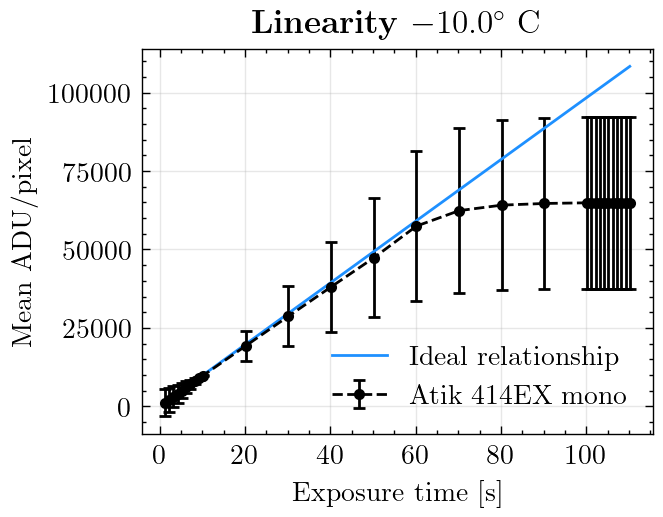
\includegraphics[width=0.58\textwidth]{/home/marc/Dropbox/STEP_Speciale_Marc/linearity.png}
%		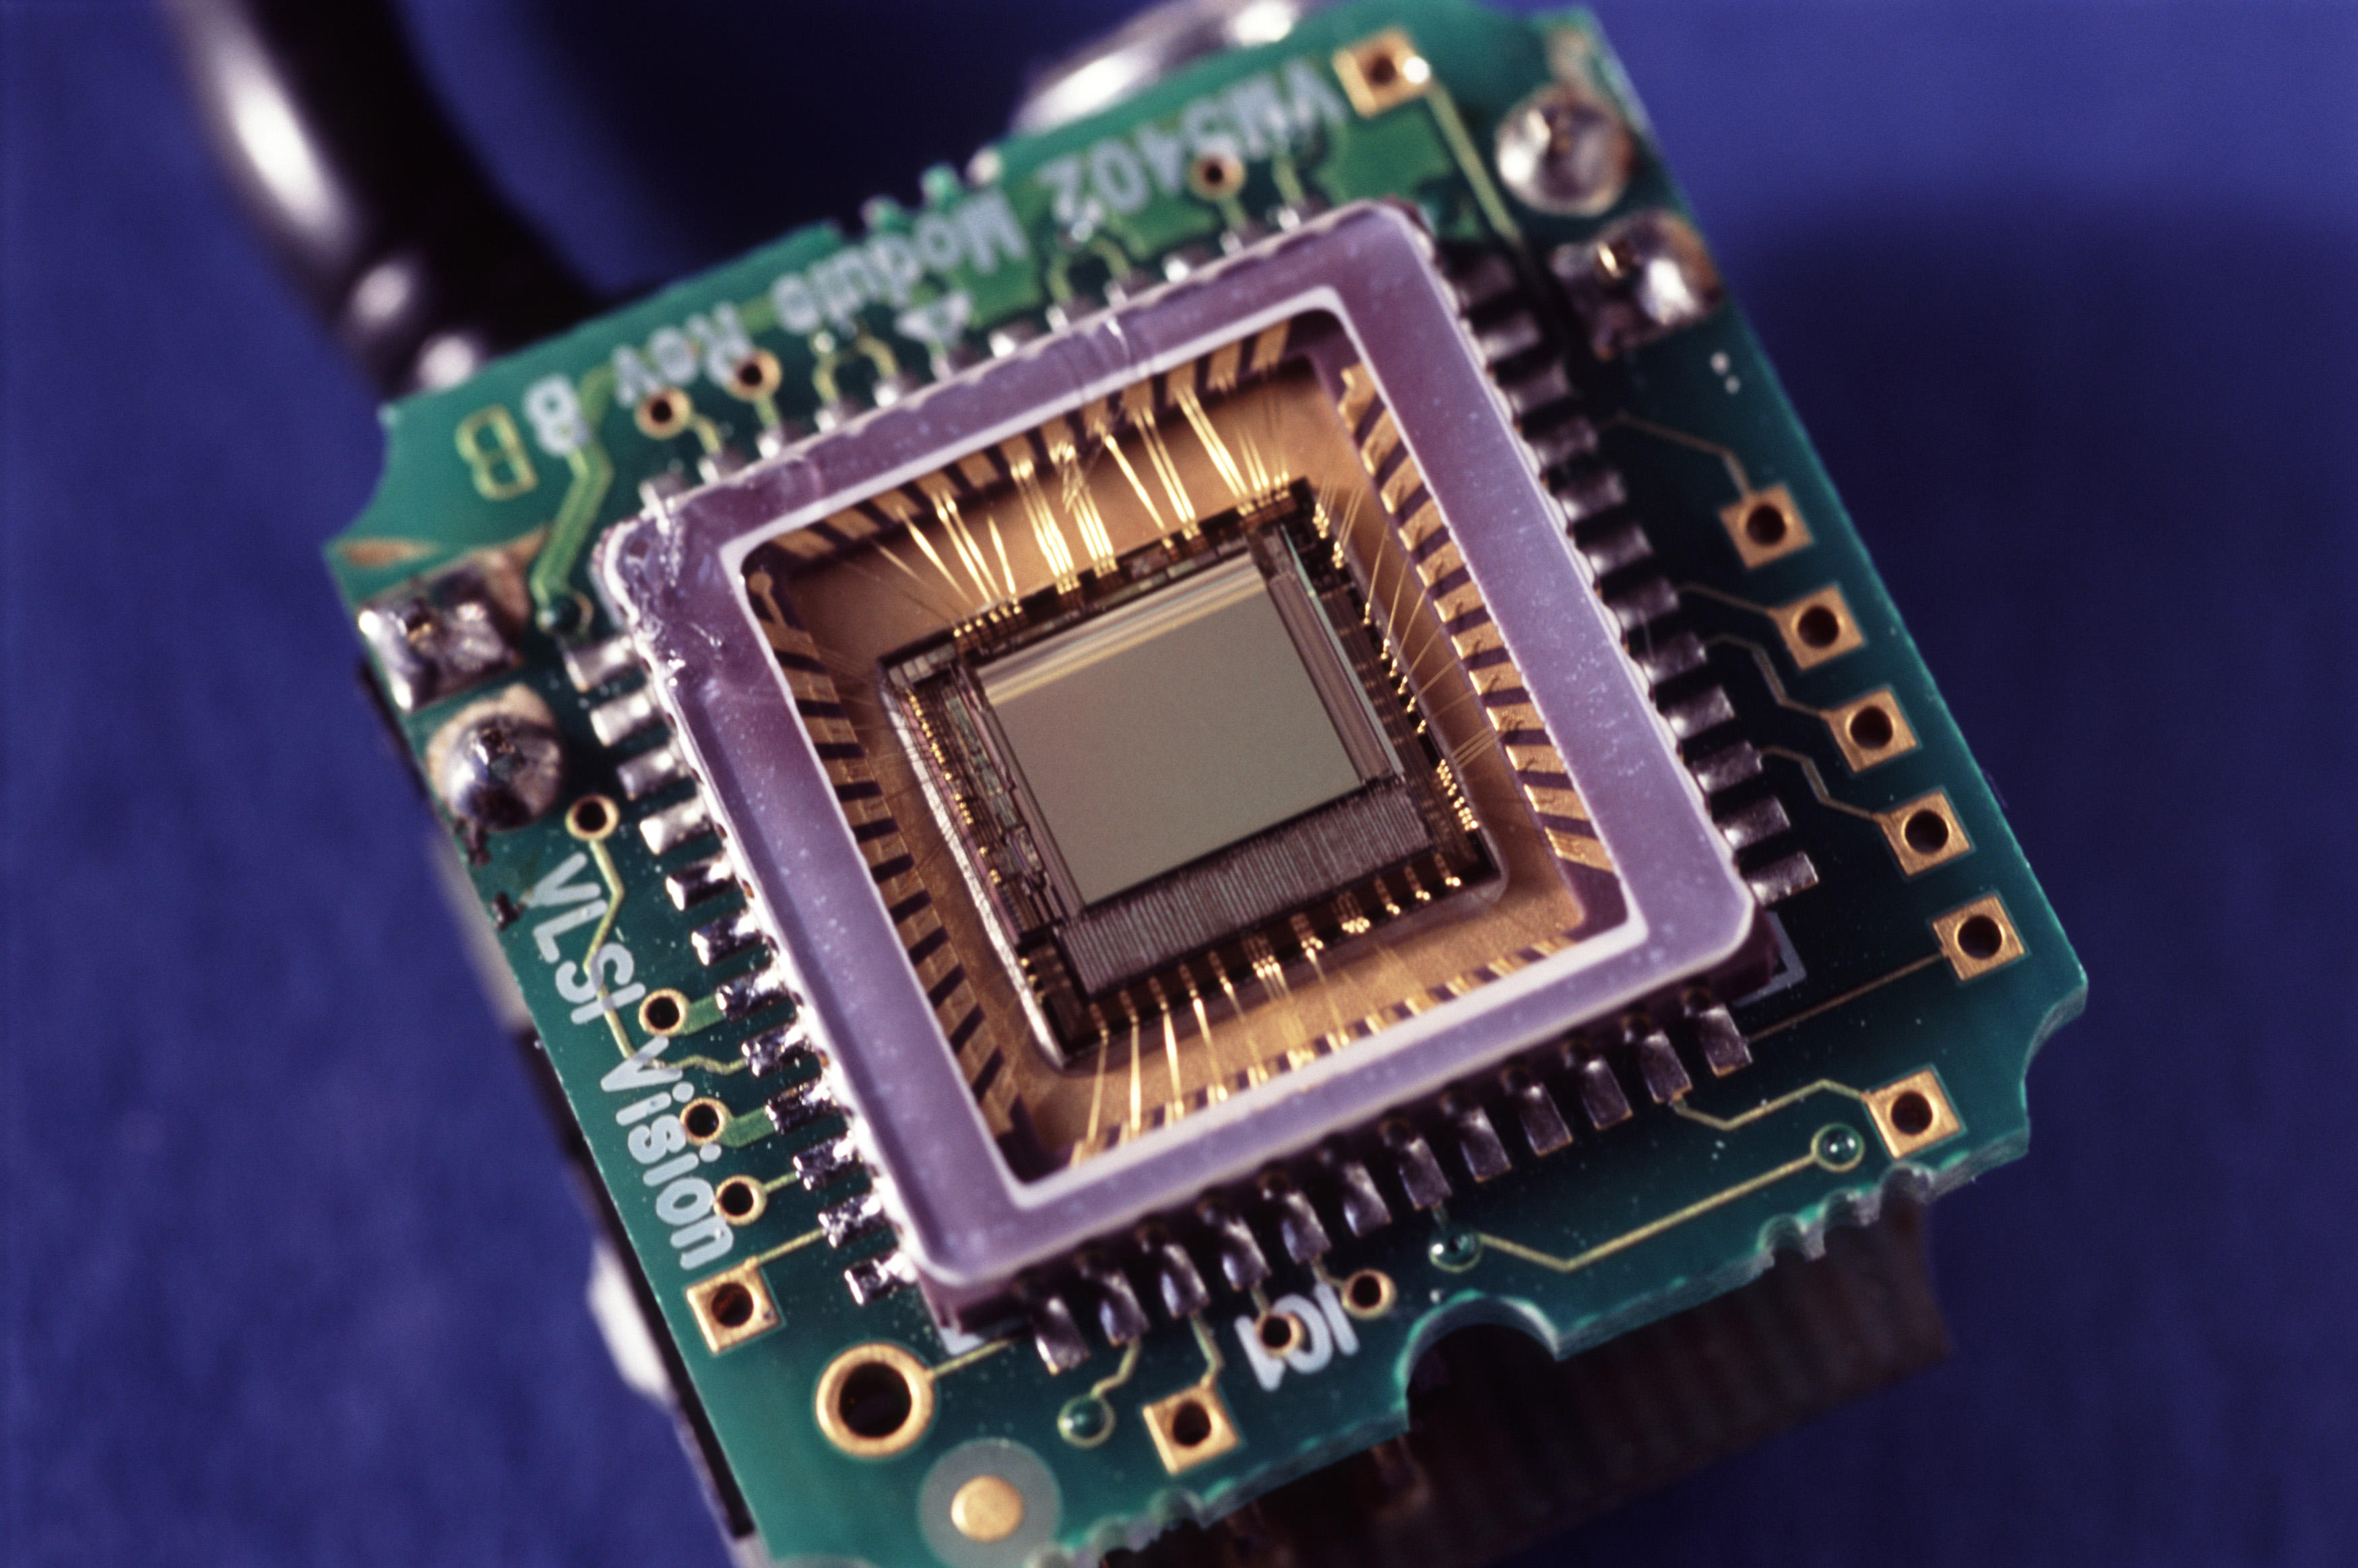
\includegraphics[width=0.8\textwidth]{ccd_sensor.jpg}
%	\end{figure}
	\thispagestyle{empty}
	
	
	\newpage
	\tableofcontents
	
	\newpage
	
	
	\subfile{sections/abstract}
	\newpage
	
	\chapter{Introduction}
	\newpage
	
	\subfile{sections/theory}
	\newpage
	
	\subfile{sections/methods}
	\newpage
	
	\subfile{sections/missionreq}
	\newpage
	
	\chapter{Results}
	\newpage
	
	\chapter{Discussion}
	\newpage
	
	\chapter{Conclusion}
	
	
	\newpage
	\bibliographystyle{plain} % We choose the &quot;plain&quot; reference style
	\bibliography{refs} % Entries are in the &quot;refs.bib&quot; file</code></pre>
	
\end{document}